\documentclass[12pt]{amsart}
\hoffset=-.90in
\textwidth=6.5in
\voffset=-.5in
\textheight=9.0in
\setlength{\parindent}{0pt}

\makeindex
\usepackage{amssymb,amsmath,amsthm}
\usepackage[all]{xy}
\usepackage{enumerate}
\usepackage{tikz}
\usetikzlibrary{calc,intersections}

\renewcommand{\1}{^{-1}}
\renewcommand{\bar}{\overline}
\newcommand{\C}{\mathbb{C}}
\newcommand{\D}{\mathbb{D}}
\newcommand{\R}{\mathbb{R}}
\newcommand{\rank}{\hbox{\rm rank}}
\renewcommand{\S}{\mathbb{S}}
\renewcommand{\setminus}{\smallsetminus}
\newcommand{\SL}{\hbox{\rm SL}} % special linear group
\newcommand{\SO}{\hbox{\rm SO}} % special orthogonal group
\newcommand{\Supp}{\hbox{\rm Supp}} % support
\newcommand{\T}{\mathbb{T}}
\renewcommand{\tilde}{\widetilde}
\newcommand{\Z}{\mathbb{Z}}

\begin{document}

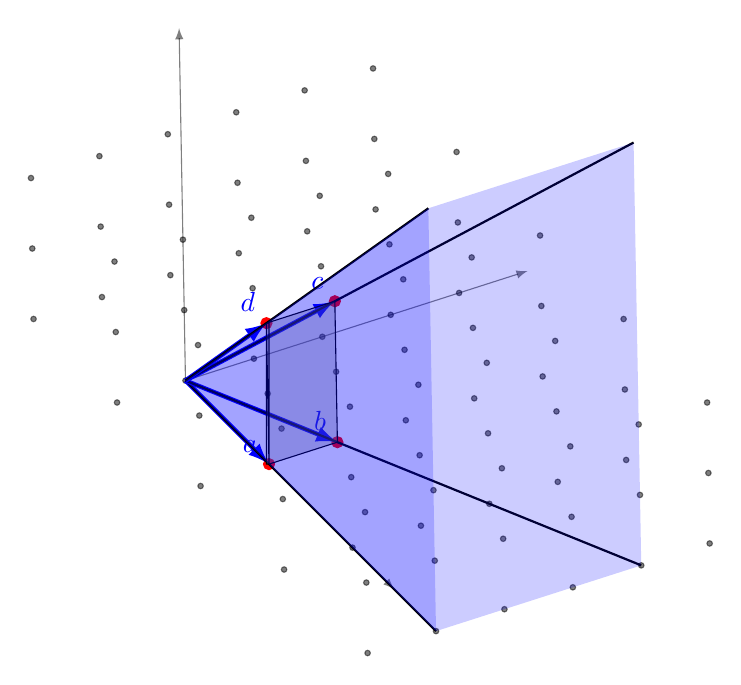
\begin{tikzpicture}
% The following is how i orient my 3d coordinate system, followed by colored axes
%[x=(-150:1),y=(-135:sqrt(2)),z=(-135:sqrt(2))]
[x=(-45:3/4),y=(35:1),z=(130:2)]
\coordinate (o) at (0,0,0);
\draw[-latex,opacity=0.5] (o)--(5,0,0);
\draw[-latex,opacity=0.5] (o)--(0,10,0);
\draw[-latex,opacity=0.5] (o)--(0,0,5);
%This is the underlying lattice:
\foreach \x in {-2,0,...,6}{
 \foreach \y in {-2,0,...,8}{
  \foreach \z in {0,...,2}{
\draw[fill,opacity=0.5](\x,\y,\z) circle[radius=1pt];}}}
%Dots relevant to the exercise:
\coordinate (a) at ($2*(1,0,0)$);
\coordinate (ta) at ($(o)!3!(a)$);
\coordinate (b) at ($2*(1,1,0)$);
\coordinate (tb) at ($(o)!3!(b)$);
\coordinate (c) at ($2*(1,1,1)$);
\coordinate (tc) at ($(o)!3!(c)$);
\coordinate (d) at ($2*(1,0,1)$);
\coordinate (td) at ($(o)!3!(d)$);
\draw[fill,color=red] (a) circle[radius=2pt];
\draw[fill,color=red] (b) circle[radius=2pt];
\draw[fill,color=red] (c) circle[radius=2pt];
\draw[fill,color=red] (d) circle[radius=2pt];

\draw [ultra thick,-latex,blue] (o) -- (a) node [above left] {$a$};
\path[name path=avect,draw,thick] (o) -- (ta);
\draw [ultra thick,-latex,blue] (o) -- (b) node [above left] {$b$};
\draw[thick] (o) -- (tb);
\draw [ultra thick,-latex,blue] (o) -- (c) node [above left] {$c$};
\draw[thick] (o) -- (tc);
\draw [ultra thick,-latex,blue] (o) -- (d) node [above left] {$d$};
\draw[thick] (o) -- (td);
\filldraw[fill=gray, fill opacity=0.3, draw=black] (a) -- (b) -- (c) -- (d) -- cycle
        rectangle (d);
\fill[fill=blue,fill opacity=0.2] (o) -- (ta) -- (tb); 
\fill[fill=blue,fill opacity=0.2] (o) -- (tb) -- (tc); 
\fill[fill=blue,fill opacity=0.2] (o) -- (tc) -- (td); 
\fill[fill=blue,fill opacity=0.2] (o) -- (td) -- (ta); 
\end{tikzpicture}

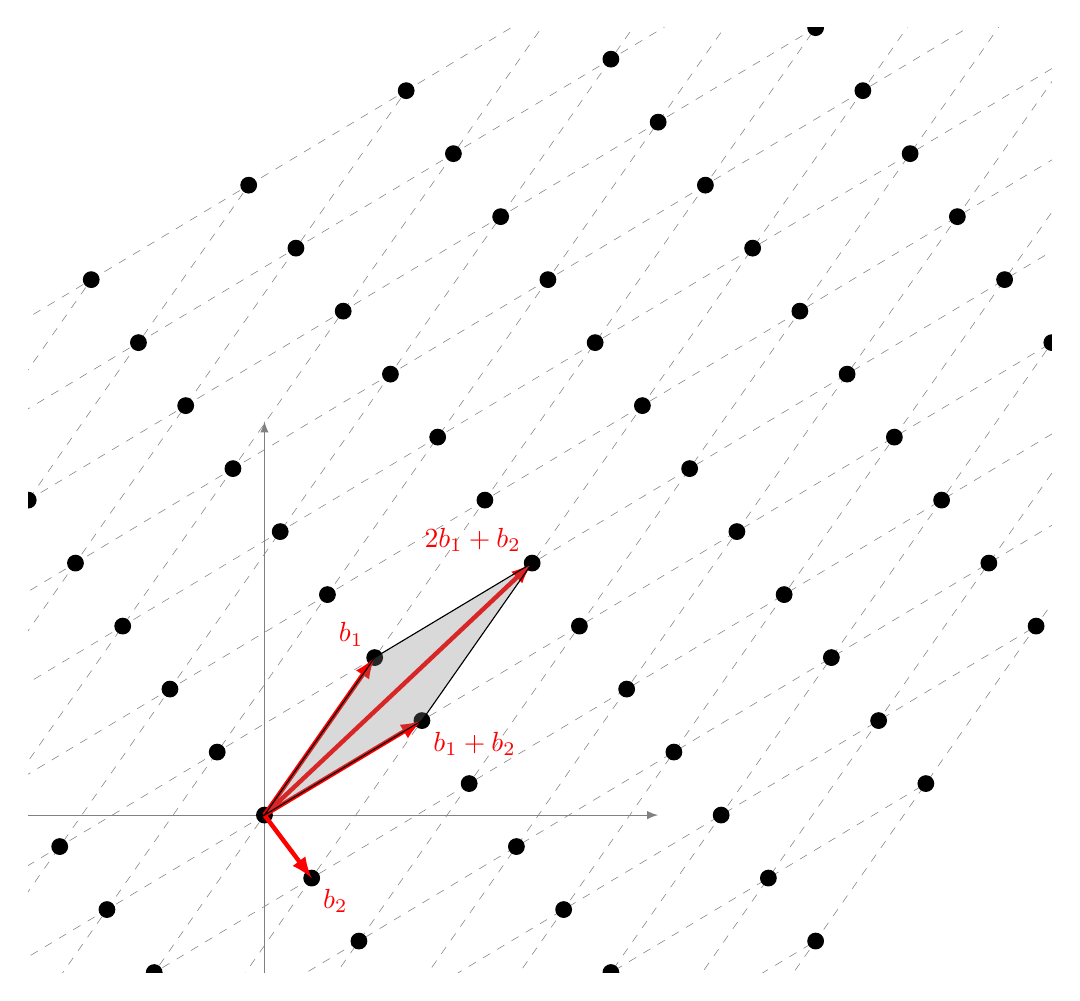
\begin{tikzpicture}
    \coordinate (Origin)   at (0,0);
    \coordinate (XAxisMin) at (-3,0);
    \coordinate (XAxisMax) at (5,0);
    \coordinate (YAxisMin) at (0,-2);
    \coordinate (YAxisMax) at (0,5);
    \draw [thin, gray,-latex] (XAxisMin) -- (XAxisMax);% Draw x axis
    \draw [thin, gray,-latex] (YAxisMin) -- (YAxisMax);% Draw y axis

    \clip (-3,-2) rectangle (10cm,10cm); % Clips the picture...
    \pgftransformcm{1}{0.6}{0.7}{1}{\pgfpoint{0cm}{0cm}}
          % This is actually the transformation matrix entries that
          % gives the slanted unit vectors. You might check it on
           % MATLAB etc. . I got it by guessing.
    \coordinate (Bone) at (0,2);
    \coordinate (Btwo) at (2,-2);
    \draw[style=help lines,dashed] (-14,-14) grid[step=2cm] (14,14);
          % Draws a grid in the new coordinates.
          %\filldraw[fill=gray, fill opacity=0.3, draw=black] (0,0) rectangle (2,2);
              % Puts the shaded rectangle
    \foreach \x in {-7,-6,...,7}{% Two indices running over each
      \foreach \y in {-7,-6,...,7}{% node on the grid we have drawn 
        \node[draw,circle,inner sep=2pt,fill] at (2*\x,2*\y) {};
            % Places a dot at those points
      }
    }
    \draw [ultra thick,-latex,red] (Origin)
        -- (Bone) node [above left] {$b_1$};
    \draw [ultra thick,-latex,red] (Origin)
        -- (Btwo) node [below right] {$b_2$};
    \draw [ultra thick,-latex,red] (Origin)
        -- ($(Bone)+(Btwo)$) node [below right] {$b_1+b_2$};
    \draw [ultra thick,-latex,red] (Origin)
        -- ($2*(Bone)+(Btwo)$) node [above left] {2$b_1+b_2$};
    \filldraw[fill=gray, fill opacity=0.3, draw=black] (Origin)
        rectangle ($2*(Bone)+(Btwo)$);
    %\draw [thin,-latex,red, fill=gray, fill opacity=0.3] (0,0)
        % -- ($2*(0,2)+(2,-2)$)
        % -- ($3*(0,2)+2*(2,-2)$) -- ($(0,2)+(2,-2)$) -- cycle;
  \end{tikzpicture}

\end{document}